\section{Validación y benchmarking}\label{tema:val}
\soporte{F2, F6, F11 y F15}

\concepto{9.1 Pirámide de pruebas}
\que Tres niveles: casos a mano (ejemplo del enunciado, sistema del enunciado y casos límite), casos aleatorios contra oráculo y comparación cruzada entre versiones (C, C++, Rust, OpenMP y CUDA).

\porque El requisito eliminatorio de CUDA obliga a demostrar la corrección, y en la entrevista te pueden pedir que lo enseñes en directo.

\como Casos límite que debe incluir \fichero{tests/casos/}:
\begin{itemize}
\item Función constante (\texttt{5}): gradiente nulo.
\item Variable que no aparece en ningún monomio: su derivada es 0.
\item Exponente 1 y exponente alto ($x^5$ en $x=1.5$).
\item Punto con $x_j=0$ (detecta el método de división) y con coordenadas negativas.
\item Coeficientes negativos y cancelación ($x-x$).
\item Monomios repetidos y variable repetida en un monomio (\texttt{xx}).
\item $M=1$, $N=1$, y $M$ no múltiplo del tamaño de bloque (comprueba el \texttt{if (m >= nMon)}).
\end{itemize}

\alt Pruebas basadas en propiedades (\emph{property-based}, con Hypothesis en Python): generan casos al azar y reducen el contraejemplo mínimo. Muy potentes para el parser; añádelas si sobra tiempo.

\concepto{9.2 Metodología de medida}
\que El protocolo para que los tiempos sean fiables y comparables (Hoefler y Belli, 2015).

\porque El análisis crítico que se evalúa solo es defendible si las medidas lo son.

\como
\begin{enumerate}
\item Máquina sin otras cargas (comprueba con \texttt{uptime} y \texttt{nvidia-smi}); anota fecha, hora y nodo.
\item Una ejecución de calentamiento no medida y después $R=10$ repeticiones.
\item Reporta mediana y desviación típica (o intervalo intercuartílico). La mediana es robusta a interferencias puntuales.
\item Afinidad fija (\texttt{OMP\_PROC\_BIND}, \texttt{OMP\_PLACES}).
\item Mismo binario y mismas opciones para todas las variantes; el secuencial de referencia, compilado igual.
\item Tiempos separados: lectura, parseo, construcción de CSC, cálculo, H2D, kernel, D2H.
\item Verificación de cada resultado medido (que la optimización no haya roto nada).
\end{enumerate}

\alt Media e intervalo de confianza al 95\,\%: también correcto si la distribución es estable, pero más sensible a valores atípicos.

\concepto{9.3 Gráficas y tablas}
\que Las representaciones de los resultados para la memoria.

\porque Una gráfica bien elegida hace evidente la conclusión.

\como Gráficas mínimas: tiempo y speedup frente a hilos (con la línea ideal y la de Amdahl), eficiencia frente a hilos, barras apiladas H2D/kernel/D2H por tamaño de problema, tiempo de kernel frente a tamaño de bloque y mapa de calor para el anidado ($h_{\text{ext}}\times h_{\text{int}}$). El prototipo \fichero{graficas.py} calcula mediana, desviación, speedup y eficiencia con Polars y dibuja con Matplotlib. Figura \ref{fig:speedup}: salida del prototipo en la máquina de nube (solo demuestra que la cadena funciona).

\begin{figure}[h]
\centering
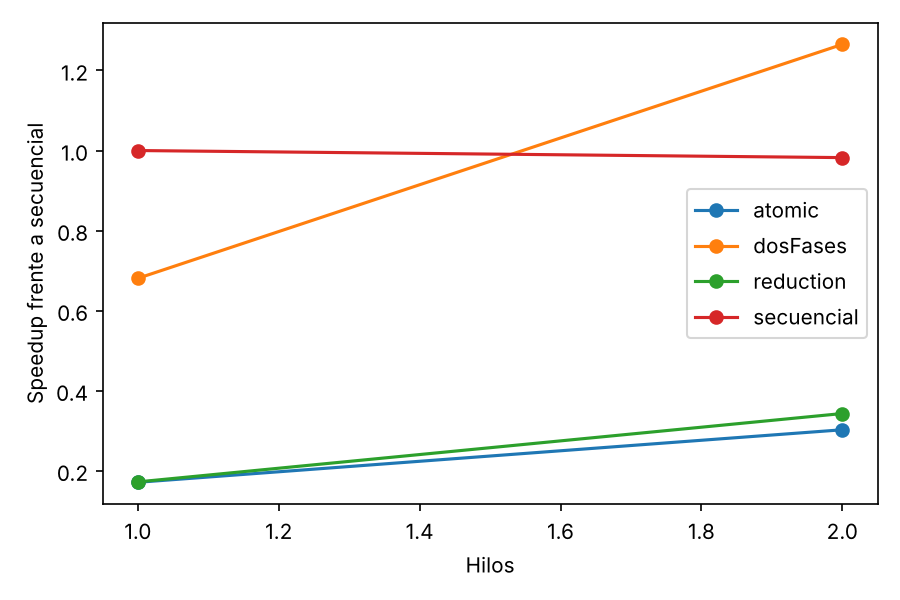
\includegraphics[width=0.62\linewidth]{figuras/speedup.png}
\caption{Speedup orientativo con 1 y 2 hilos (nube de 2 vCPU, $N=10^3$, $M=10^5$). No usar en la memoria.}
\label{fig:speedup}
\end{figure}

\alt Gnuplot, o pgfplots dentro de LaTeX (mejor integración tipográfica, más lento de iterar).

\section{Herramientas y entorno}\label{tema:herr}
\soporte{F0, F12 y F15}

\concepto{10.1 Git e identidad de autor}
\que Control de versiones. Cada commit guarda autor y \emph{committer}.

\porque Quieres que solo figures tú en el repositorio, y el enunciado valora mostrar la evolución incremental del código.

\como Configura una vez \texttt{git config user.name "Antonio Millán Rodríguez"} y \texttt{git config user.email "antoniomillanr45@gmail.com"}. Un commit por fase, con un mensaje que nombre la fase, y una etiqueta por punto de control (\texttt{git tag pc1}). Verifica la autoría con:
\begin{lstlisting}[language=bash]
git log --format='%an <%ae> | %cn <%ce>'
git log --format=%B | grep -iE "co-authored|claude"
\end{lstlisting}
El segundo comando no debe devolver nada. La rama \texttt{claude/fervent-bell-1ekfj8} tiene un commit con autor \emph{Claude}: si la fusionas, rehaz ese commit con tu identidad (\texttt{git cherry-pick} y \texttt{git commit --amend --reset-author}) en lugar de fusionarlo tal cual, y borra la rama remota.

\alt Ramas por fase con \emph{pull requests}: más ordenado, pero excesivo para un proyecto individual.

\concepto{10.2 Make}
\que Herramienta que recompila solo lo que ha cambiado según reglas de dependencias.

\porque Un \texttt{make all} y un \texttt{make test} son lo que el profesor ejecutará en el servidor.

\como Ver \fichero{docs/guia/codigo/Makefile} (probado): objetivos \texttt{all}, \texttt{grad}, \texttt{test} y \texttt{clean}, con \texttt{ARCH = -arch=sm\_89} como variable que se cambia en el servidor (\texttt{make grad ARCH=-arch=sm\_80}).

\alt CMake: detecta CUDA y OpenMP de forma portable, pero añade una capa de complejidad innecesaria para un proyecto de 10 ficheros.

\concepto{10.3 Contenedores: Docker y Apptainer}
\que Un contenedor empaqueta el sistema, las dependencias y el binario. Docker es el estándar general; Apptainer (antes Singularity; Kurtzer et al., 2017) es el habitual en servidores HPC porque no exige privilegios de \texttt{root}.

\porque El enunciado pide \emph{incluir la solución en un sistema de contenedores}, y sirve para fijar versiones (reproducibilidad).

\como Dockerfile orientativo (\fichero{docs/guia/codigo/Dockerfile}; no se ha podido construir en este entorno; etiqueta de imagen y compatibilidad de versiones con Ubuntu 22.04 \pv):
\begin{lstlisting}
FROM nvidia/cuda:12.4.1-devel-ubuntu22.04
RUN apt-get update && apt-get install -y --no-install-recommends make python3 python3-pip && rm -rf /var/lib/apt/lists/*
RUN pip3 install --no-cache-dir sympy==1.14.0 numpy==2.5.3 polars==2.1.0 matplotlib==3.11.2
WORKDIR /app
COPY . .
RUN make all grad
CMD ["make", "test"]
\end{lstlisting}
Ejecución con GPU: \texttt{docker run --gpus all imagen}; requiere NVIDIA Container Toolkit en el anfitrión. Con Apptainer: \texttt{apptainer build grad.sif docker-daemon://imagen:latest} y \texttt{apptainer run --nv grad.sif}.

\alt Podman (Docker sin demonio y sin \texttt{root}) o un entorno \texttt{conda}/\texttt{venv} más un \texttt{Makefile}: no es un contenedor y no cumple la tarea 6.

\begin{trampa}
La versión de CUDA de la imagen no puede ser más nueva de lo que admite el driver del servidor. Mira \texttt{nvidia-smi} (``CUDA Version'') antes de elegir la etiqueta.
\end{trampa}

\concepto{10.4 Librerías de Python}
\begin{center}\small
\begin{tabularx}{\linewidth}{@{}l l X@{}}
\toprule
Librería & Papel & Por qué sí o por qué no como base \\
\midrule
SymPy 1.14 & Validación (oráculo) & Exacta, pero lenta para $M>10^4$: solo casos pequeños \\
NumPy 2.5 & Generación & Generación vectorizada de enteros aleatorios con \texttt{default\_rng} \\
Polars 2.1 & Generación y análisis & Agregaciones rápidas de CSV de tiempos; Pandas también valdría \\
Matplotlib 3.11 & Análisis & Gráficas para la memoria \\
JAX o PyTorch & Comparación opcional & AD de referencia del estado del arte; no son base porque el enunciado pide C \\
\bottomrule
\end{tabularx}
\end{center}
Versiones probadas en esta guía; fíjalas en \fichero{requirements.txt}.

\concepto{10.5 Trabajo en el servidor de prácticas}
\que El entorno donde se harán las pruebas finales.

\porque Es obligatorio, y su hardware determina todos los resultados.

\como Copia con \texttt{git clone} (o \texttt{rsync}), compila allí con \texttt{ARCH} adaptado y lanza los benchmarks con \texttt{nohup ./reproduce.sh \&} o dentro de \texttt{tmux}. Si hay gestor de colas (Slurm), usa \texttt{sbatch} y pide los nodos en exclusiva \pv.

\alt Medir en el portátil sirve para desarrollar y como segundo entorno comparativo en la memoria, pero no sustituye al servidor.

\section{IA generativa, prompts y memoria}\label{tema:ia}
\soporte{F13 y F14 (apartados 2.1.4 y 2.1.5, 30\,\% en total)}

\concepto{11.1 Ingeniería de prompts}
\que Diseñar la petición a un modelo de lenguaje para obtener una respuesta útil: contexto, objetivo, restricciones, formato de salida y ejemplos.

\porque Se puntúa \emph{la calidad y el contexto} de los prompts y su refinamiento incremental.

\como Estructura de prompt que funciona para código:
\begin{enumerate}
\item Rol y contexto: asignatura, enunciado y estado actual del código (adjunto).
\item Tarea concreta y criterio de éxito verificable (``debe dar (8, 15, 8)'').
\item Restricciones: C11, OpenMP 4.5, sin comentarios, nomenclatura, sin dependencias.
\item Formato: solo el fichero, o un diff.
\item Iteración: pega el error de compilación o los tiempos medidos y pide un diagnóstico, no solo un arreglo.
\end{enumerate}
Ejemplo de refinamiento: ``paraleliza el gradiente con OpenMP'' $\rightarrow$ ``paraleliza \texttt{gradSec} sobre CSR con OpenMP evitando atómicos; propone dos variantes y explica su coste en memoria'' $\rightarrow$ ``la variante \emph{reduction} es 3 veces más lenta que el secuencial con 2 hilos; aquí están los tiempos; ¿por qué?''.

\alt Usar la IA solo para depurar o documentar (más seguro, menos material para el apartado). Lo valorado es mostrar el proceso completo, incluidas las respuestas erróneas y cómo las detectaste.

\concepto{11.2 Registro de interacciones}
\que Un diario en \fichero{docs/prompts.md}.

\porque Reconstruirlo al final es costoso y poco creíble. El enunciado pide, para cada IA: ámbito de uso, lista de prompts, soluciones obtenidas y valoración final.

\como Plantilla por entrada:
\begin{lstlisting}
## Fecha  IA y modelo  Fase
Prompt: ...
Respuesta resumida: ...
Fragmento clave: ...
Problema detectado y cómo: ...
Commit resultante: ...
\end{lstlisting}
Incluye esta guía como una interacción (ámbito: planificación y estudio).

\alt Exportar las conversaciones completas como anexo: útil como respaldo, pero el cuerpo de la memoria debe ser un análisis, no un volcado.

\concepto{11.3 Memoria con el esquema oficial}
\que El documento de entrega: Abstract, Introducción, El problema, Paralelización (secuencial, multinúcleo, GPU, extensiones), Resultados (entorno, resultados), Conclusiones y Bibliografía.

\porque Vale un 15\,\% y es lo que se lee antes de la entrevista.

\como Cada tema de esta guía alimenta una sección: 1 y 2 van a ``El problema''; 3, 5, 6, 7 y 8, a ``Paralelización''; 4 y 9, a ``Resultados''; 12, a ``Introducción''. Escribe cada sección al cerrar su fase, no al final. Cita solo referencias que hayas consultado.

\alt LaTeX (recomendado: fórmulas y bibliografía) o Markdown con Pandoc (más rápido, menos control).

\section{Estado del arte}\label{tema:arte}
\soporte{F14 (introducción) y contexto de todas}

\concepto{12.1 Diferenciación automática}
\que La técnica estándar para gradientes en aprendizaje automático y optimización (Baydin et al., 2018; Griewank y Walther, 2008). El modo inverso calcula el gradiente completo con un coste acotado por un pequeño múltiplo constante del coste de evaluar $f$ (principio del gradiente barato).

\porque Sitúa el proyecto: nuestro algoritmo prefijo-sufijo es un modo inverso especializado para productos, sin cinta (\emph{tape}) ni grafo, gracias a conocer la estructura polinómica.

\como Herramientas: PyTorch (\texttt{autograd}; Paszke et al., 2019), JAX (\texttt{grad}, \texttt{jit}, \texttt{vmap}; Bradbury et al., 2018), Enzyme (AD a nivel de LLVM, incluso de kernels CUDA; Moses y Churavy, 2020) y CasADi. Un experimento opcional valioso: comparar tu CUDA con \texttt{jax.grad} sobre el mismo polinomio en la misma GPU.

\alt --- (es el contexto, no una opción de implementación).

\concepto{12.2 Evaluación de polinomios y sus derivadas en GPU}
\que Existe trabajo específico sobre evaluar y diferenciar sistemas polinómicos en GPU para métodos de homotopía, por ejemplo Verschelde y Yoffe (2012) \pv. Usan, entre otras ideas, productos tipo Speelpenning para los monomios.

\porque Confirma que el planteamiento (monomio por hilo y productos prefijo y sufijo) es el adecuado y da una referencia seria para la introducción.

\como Lee el resumen y la sección de algoritmo antes de citarlo. Si no puedes acceder, no lo cites.

\alt SpMV en GPU (Bell y Garland, 2009) es el problema hermano: mismo patrón disperso, mismas técnicas (CSR, ELL, \emph{sliced} ELL). Sus conclusiones sobre formatos son directamente aplicables.

\concepto{12.3 En qué se diferencia este proyecto}
\begin{itemize}
\item Derivación exacta especializada en polinomios dispersos, sin grafo de AD: menos memoria y sin dependencias.
\item Comparación sistemática de estrategias de acumulación (\emph{reduction}, \emph{atomic}, dos fases) en CPU y GPU sobre el mismo problema.
\item Extensión al Jacobiano con un CSR global y estudio de anidado.
\item Documentación del uso de IA generativa como parte del método.
\end{itemize}
No es más rápido que una biblioteca de AD en general: es más rápido \emph{en este caso particular}, y eso es lo que hay que demostrar con medidas.
\clearpage
